%% Integration with calendaring
\pgfkeys{/tikz/flag-flying day/.code =
  {
    \draw (-\cellwidth,0) node [above right,font=\Huge]
    {\hspace*{-.2cm}\resizebox{!}{0.8ex}{\usebox{\flagRU}}};
  }
}

\pgfkeys{/tikz/flag-victory day/.code =
  {
    \draw (-\cellwidth,0) node [above right,font=\Huge]
    {\resizebox{!}{1.75ex}{\flagVictory}};
  }
}

\pgfkeys{/tikz/flag-navy day/.code =
  {
    \draw (-\cellwidth,0) node [above right,font=\Huge]
    {\resizebox{!}{0.8ex}{\flagRusNavy}};
  }
}

\pgfkeys{/tikz/flag-airborne day/.code =
  {
    \draw (-\cellwidth,0) node [above right,font=\Huge]
    {\resizebox{!}{0.8ex}{\flagRusAirborne}};
  }
}

\pgfkeys{/tikz/flag-military day/.code =
  {
    \draw (-\cellwidth,0) node [above right,font=\Huge]
    {\resizebox{!}{0.8ex}{\usebox{\flagRusDefence}}};
  }
}

\pgfkeys{/tikz/flag-orthodox day/.code =
  {
    \draw (-\cellwidth,0) node [above right,font=\Huge]
    {\resizebox{!}{0.8ex}{\usebox{\OrthodoxChrist}}};
  }
}


%% Flag of Russia
\definecolor{myred}{RGB}{216,30,5}
\definecolor{myblue}{RGB}{0,81,186}

\newsavebox{\flagRU}
\savebox{\flagRU}{
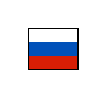
\begin{tikzpicture}
\fill[myred] rectangle (18pt,5pt);
\fill[myblue,yshift=5pt] rectangle (18pt,5pt);
\draw rectangle (18pt,15pt);
\end{tikzpicture}
}

%% Flag of Russian Navy
\definecolor{cfff}{RGB}{255,255,255}
\definecolor{c0039a6}{RGB}{0,57,166}

\newcommand{\flagRusNavy}{%

\begin{tikzpicture}[y=0.80pt,x=0.80pt,yscale=-1, inner sep=0pt, outer sep=0pt]
% rect3037
\path[fill=cfff,rounded corners=0.0000cm] (0.0000,0.0000) rectangle
  (30.0000,20.0000);
% path3039
\path[draw=c0039a6,line width=2.400pt] (0.0000,0.0000) --
  (30.0000,20.0000)(0.0000,20.0000) -- (30.0000,0.0000);
\end{tikzpicture}}

%% Orthodoxy christ 
\definecolor{cffffff}{RGB}{255,255,255}
\newsavebox{\OrthodoxChrist}
\savebox{\OrthodoxChrist}{%
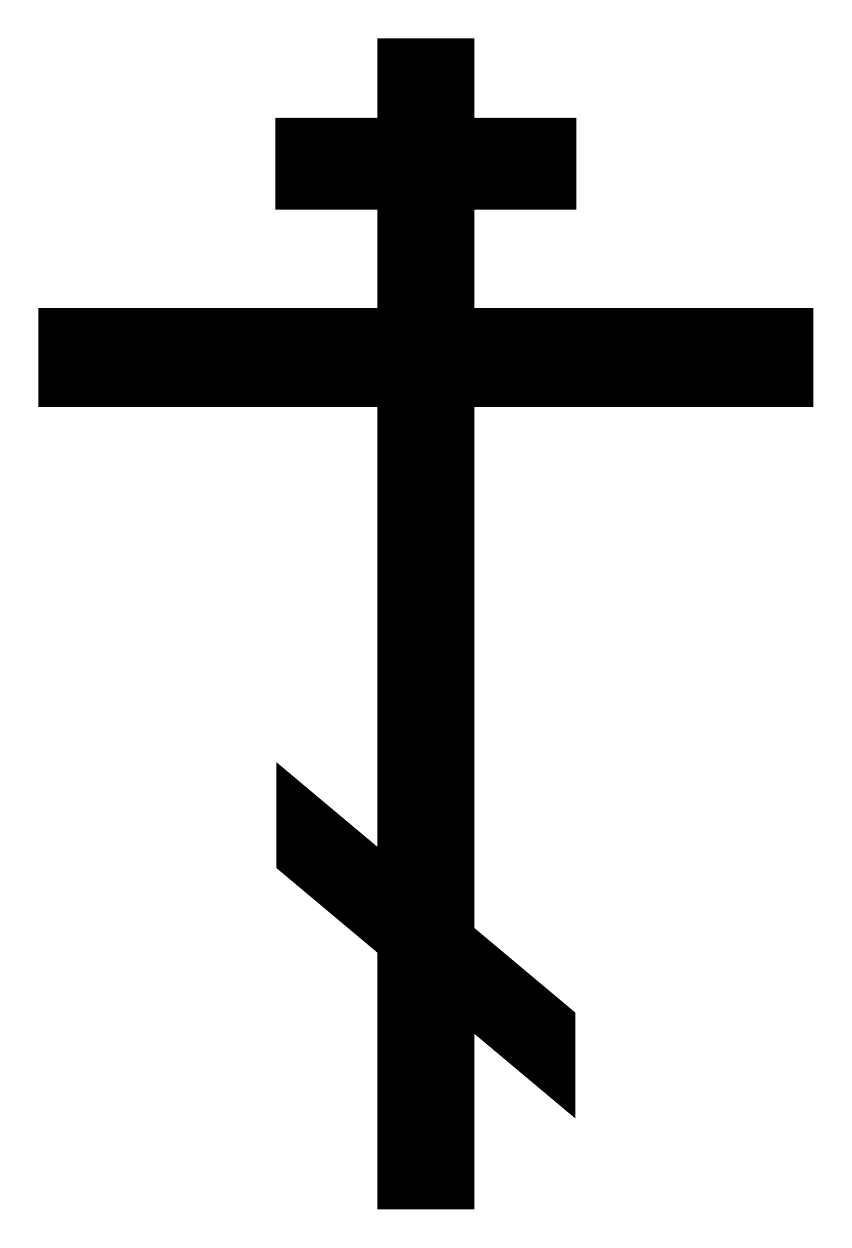
\begin{tikzpicture}[y=0.80pt,x=0.80pt,yscale=-1, inner sep=0pt, outer sep=0pt]
% path4649
\path[fill=black] (173.1250,21.0938) -- (173.1250,57.0312) -- (127.0312,57.0312)
  -- (127.0312,98.4375) -- (173.1250,98.4375) -- (173.1250,142.9688) --
  (20.0000,142.9688) -- (20.0000,187.5000) -- (173.1250,187.5000) --
  (173.1250,386.2812) -- (127.4375,348.0000) -- (127.4375,395.7188) --
  (173.1250,434.0000) -- (173.1250,550.0000) -- (216.8750,550.0000) --
  (216.8750,470.6250) -- (262.5938,508.9375) -- (262.5938,461.2188) --
  (216.8750,422.9062) -- (216.8750,187.5000) -- (370.0000,187.5000) --
  (370.0000,142.9688) -- (216.8750,142.9688) -- (216.8750,98.4375) --
  (262.9688,98.4375) -- (262.9688,57.0312) -- (216.8750,57.0312) --
  (216.8750,21.0938) -- (173.1250,21.0938) -- cycle;

% path6400
\path[fill=cffffff] (173.1250,16.2500) .. controls (170.4513,16.2536) and
  (168.2848,18.4201) .. (168.2812,21.0938) -- (168.2812,52.1875) --
  (127.0312,52.1875) .. controls (124.3576,52.1911) and (122.1911,54.3576) ..
  (122.1875,57.0312) -- (122.1875,98.4375) .. controls (122.1911,101.1111) and
  (124.3576,103.2777) .. (127.0312,103.2812) -- (168.2812,103.2812) --
  (168.2812,138.1250) -- (20.0000,138.1250) .. controls (17.3263,138.1286) and
  (15.1598,140.2951) .. (15.1562,142.9688) -- (15.1562,187.5000) .. controls
  (15.1598,190.1737) and (17.3263,192.3402) .. (20.0000,192.3438) --
  (168.2812,192.3438) -- (168.2812,375.8750) -- (130.5625,344.2812) .. controls
  (129.1181,343.0687) and (127.1018,342.8033) .. (125.3929,343.6008) .. controls
  (123.6839,344.3983) and (122.5922,346.1141) .. (122.5938,348.0000) --
  (122.5938,395.7188) .. controls (122.5894,397.1513) and (123.2185,398.5126) ..
  (124.3125,399.4375) -- (168.2812,436.2812) -- (168.2812,550.0000) .. controls
  (168.2848,552.6736) and (170.4513,554.8402) .. (173.1250,554.8438) --
  (216.8750,554.8438) .. controls (219.5487,554.8402) and (221.7152,552.6736) ..
  (221.7188,550.0000) -- (221.7188,481.0312) -- (259.4688,512.6562) .. controls
  (260.9131,513.8688) and (262.9294,514.1342) .. (264.6384,513.3367) .. controls
  (266.3473,512.5392) and (267.4391,510.8234) .. (267.4375,508.9375) --
  (267.4375,461.2188) .. controls (267.4419,459.7862) and (266.8127,458.4249) ..
  (265.7188,457.5000) -- (221.7188,420.6250) -- (221.7188,192.3438) --
  (370.0000,192.3438) .. controls (372.6737,192.3402) and (374.8402,190.1737) ..
  (374.8438,187.5000) -- (374.8438,142.9688) .. controls (374.8402,140.2951) and
  (372.6737,138.1286) .. (370.0000,138.1250) -- (221.7188,138.1250) --
  (221.7188,103.2812) -- (262.9688,103.2812) .. controls (265.6424,103.2777) and
  (267.8089,101.1111) .. (267.8125,98.4375) -- (267.8125,57.0312) .. controls
  (267.8089,54.3576) and (265.6424,52.1911) .. (262.9688,52.1875) --
  (221.7188,52.1875) -- (221.7188,21.0938) .. controls (221.7152,18.4201) and
  (219.5487,16.2536) .. (216.8750,16.2500) -- (173.1250,16.2500) -- cycle;

% rect1389
\path[fill=black] (173.1250,21.0938) -- (173.1250,57.0312) -- (127.0312,57.0312)
  -- (127.0312,98.4375) -- (173.1250,98.4375) -- (173.1250,142.9688) --
  (20.0000,142.9688) -- (20.0000,187.5000) -- (173.1250,187.5000) --
  (173.1250,386.2812) -- (127.4375,348.0000) -- (127.4375,395.7188) --
  (173.1250,434.0000) -- (173.1250,550.0000) -- (216.8750,550.0000) --
  (216.8750,470.6250) -- (262.5938,508.9375) -- (262.5938,461.2188) --
  (216.8750,422.9062) -- (216.8750,187.5000) -- (370.0000,187.5000) --
  (370.0000,142.9688) -- (216.8750,142.9688) -- (216.8750,98.4375) --
  (262.9688,98.4375) -- (262.9688,57.0312) -- (216.8750,57.0312) --
  (216.8750,21.0938) -- (173.1250,21.0938) -- cycle;
\end{tikzpicture}}

%% Flag of the Russian Arborne Troops
\newcommand{\flagRusAirborne}{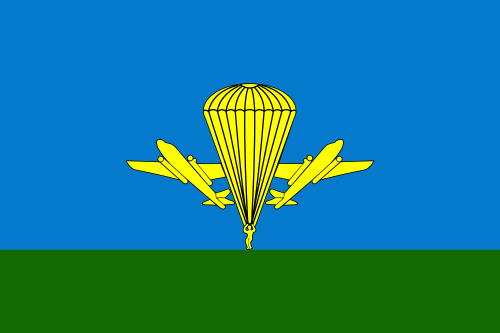
\includegraphics{flags/RusAirborne.png}}

%% Flag of the Russian Ministry of Defence
\newsavebox{\flagRusDefence}
\savebox{\flagRusDefence}{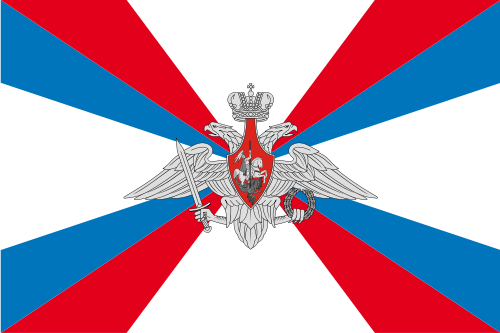
\includegraphics{flags/RusDefence.png}}

%% Saint George ribbon - Vicory Day. 9, May.
\newcommand{\flagVictory}{\rotatebox{90}{
\includegraphics{flags/9May.png}}}
